%%
% This is an Overleaf template for presentations
% using the TUM Corporate Desing https://www.tum.de/cd
%
% For further details on how to use the template, take a look at our
% GitLab repository and browse through our test documents
% https://gitlab.lrz.de/latex4ei/tum-templates.
%
% The tumbeamer class is based on the beamer class.
% If you need further customization please consult the beamer class guide
% https://ctan.org/pkg/beamer.
% Additional class options are passed down to the base class.
%
% If you encounter any bugs or undesired behaviour, please raise an issue
% in our GitLab repository
% https://gitlab.lrz.de/latex4ei/tum-templates/issues
% and provide a description and minimal working example of your problem.
%%

\documentclass{setbeamer}

\usepackage{pdfpages}

% presentation metadata
\title{Markup Languages}
\subtitle{\LaTeX{} und Markdown}

\institute{\theChairName\\\theDepartmentName\\\theUniversityName}
\date[05.10.2023]{5. Oktober 2023}

\footline{\insertauthor~|~\insertshorttitle~|~\insertshortdate}

\begin{document}

\maketitle

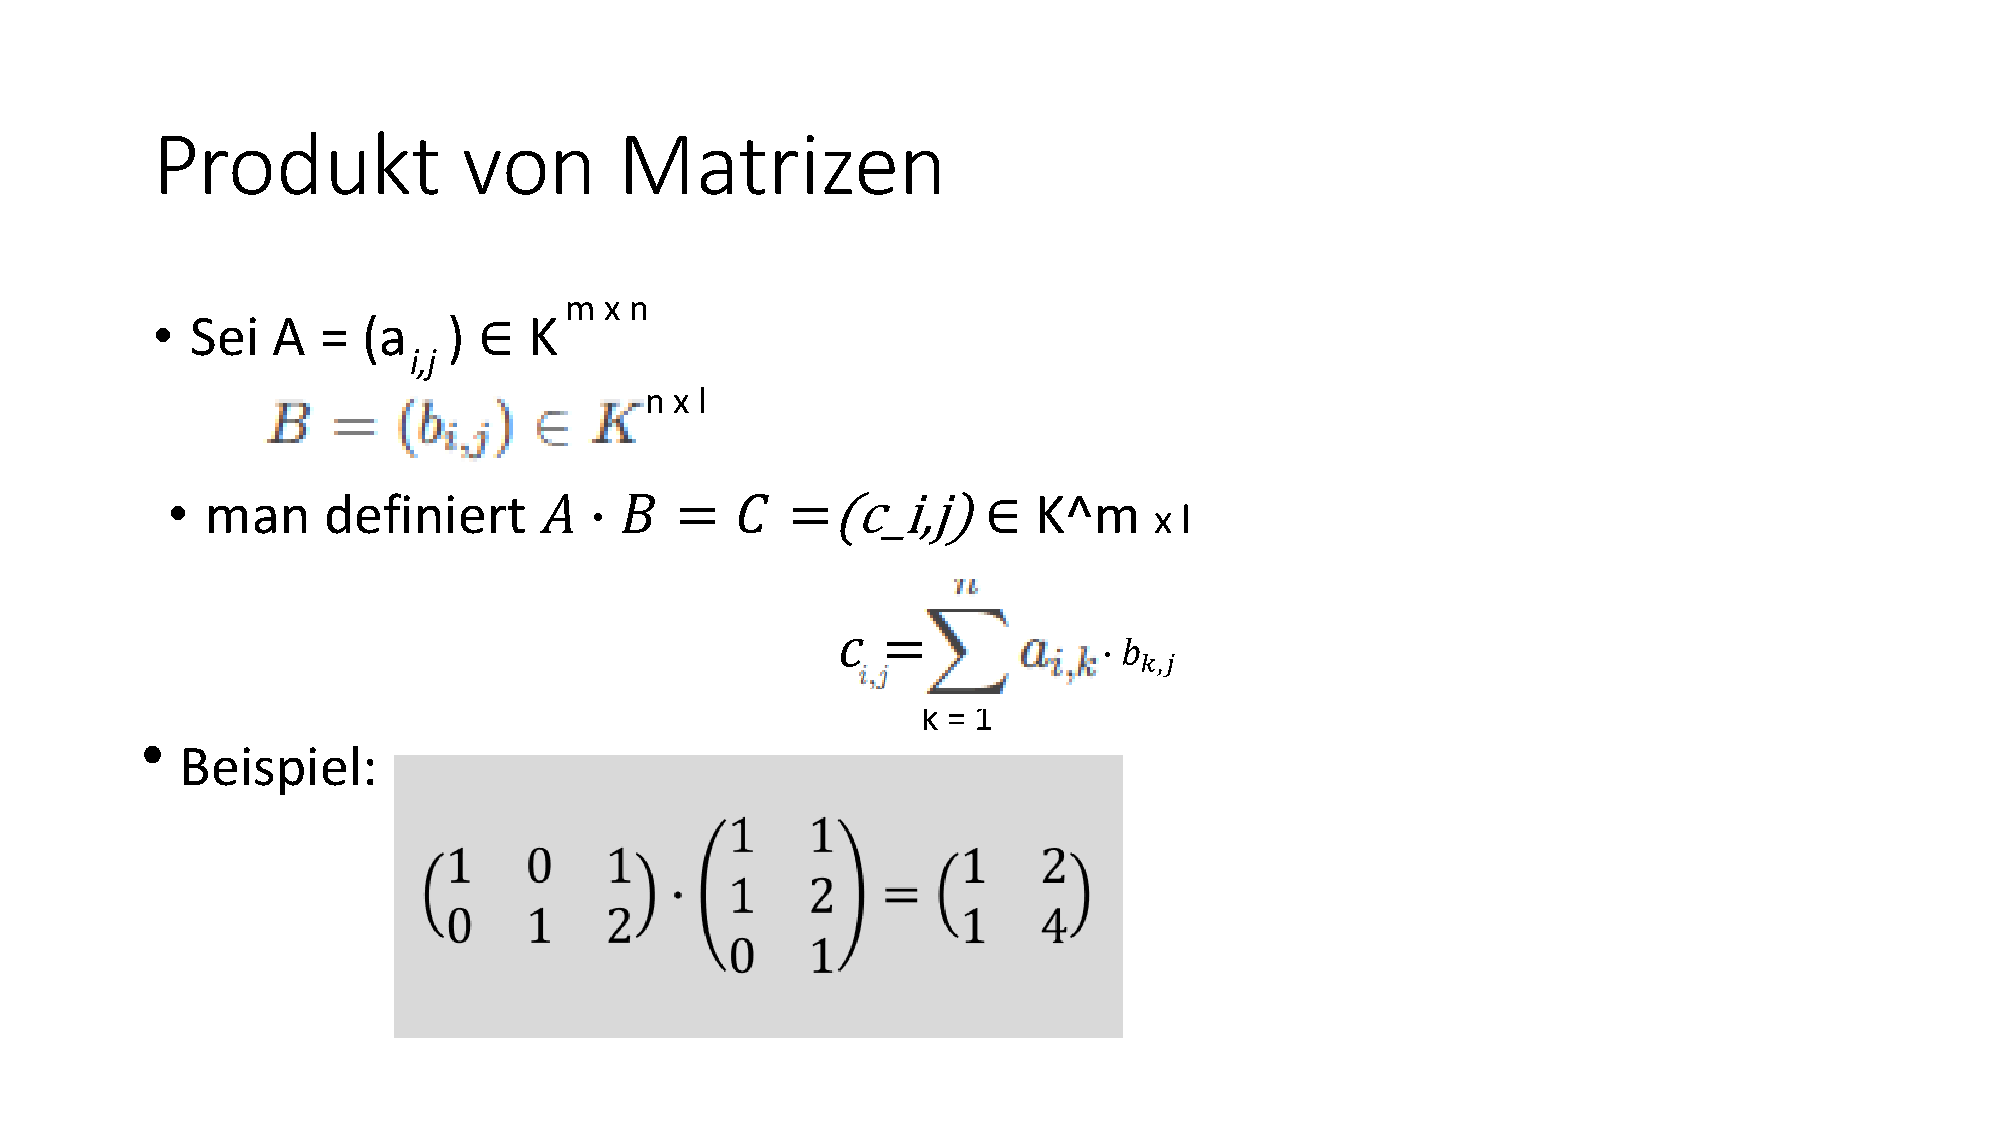
\includepdf[pages=-]{resources/WYSIWYG_example.pdf}

\section{WYSIWYG vs. WYSIWYM}
\begin{frame}{WYSIWYG}{What You See Is What You Get}
    Graphische Editors, die einem das Anzeigen, was am Ende raus kommt.

    \pause
    Beispiele:
    \begin{columns}
        \begin{column}{0.25\textwidth}
            \begin{itemize}
                \item Microsoft Word
                \item Microsoft Powerpoint
            \end{itemize}
        \end{column}

        \begin{column}{0.25\textwidth}
            \begin{itemize}
                \item Google Sheets
                \item Google Slides
            \end{itemize}
        \end{column}

        \begin{column}{0.25\textwidth}
            \begin{itemize}
                \item Apple Pages
                \item Apple Keynote
            \end{itemize}
        \end{column}

        \begin{column}{0.25\textwidth}
            \begin{itemize}
                \item LibreOffice Writer
                \item LibreOffice Impress
            \end{itemize}
        \end{column}
    \end{columns}

    \pause
    \vspace{3mm}
    \begin{columns}
        \begin{column}{0.5\textwidth}
            Vorteile:
            \begin{itemize}
                \item leichte Bedienung
                \item direktes Feedback beim editieren
            \end{itemize}
        \end{column}

        \pause
        \begin{column}{0.5\textwidth}
            Nachteile:
            \begin{itemize}
                \item oft ungenau
                \item Fehler kann man nur visuell erkennen
            \end{itemize}
        \end{column}
    \end{columns}
\end{frame}

\begin{frame}{WYSIWYM}{What You See Is What You Mean}
    Spezifikation, wie das Endergebnis aussehen soll.
    \pause
    \begin{columns}
        \begin{column}{0.5\textwidth}
            Beispiele:
            \begin{itemize}
                \item \TeX{} bzw. \LaTeX{}
                \item troff bzw. groff
            \end{itemize}
        \end{column}

        \begin{column}{0.5\textwidth}
            \begin{itemize}
                \item HTML
                \item Markdown
                \item reStructuredText
                \item Asciidoc
            \end{itemize}
        \end{column}
    \end{columns}

    \pause
    \vspace{3mm}
    \begin{columns}
        \begin{column}{0.5\textwidth}
            Vorteile:
            \begin{itemize}
                \item meistens Text-basiert (leichtes version control mit z. B. git)
                \item ``Korrektheit'' kann sichergestellt werden
            \end{itemize}
        \end{column}

        \pause
        \begin{column}{0.5\textwidth}
            Nachteile:
            \begin{itemize}
                \item hohe Learning Curve
                \item kein (oder nur langsames) visuelles Feedback
            \end{itemize}
        \end{column}
    \end{columns}
\end{frame}

\section{\LaTeX{}}
\begin{frame}{\LaTeX{} Begriffe}
    \pause
    \begin{columns}
        \begin{column}{0.5\textwidth}
            Syntax:
            \begin{itemize}
                \item \TeX{}
                \item \LaTeX{}
            \end{itemize}
        \end{column}

        \pause
        \begin{column}{0.5\textwidth}
            Compiler:
            \begin{itemize}
                \item \TUMCodeInline{sh}{latex}
                \item \TUMCodeInline{sh}{pdflatex}
                \item \TUMCodeInline{sh}{xelatex}
                \item (\TUMCodeInline{sh}{latexmk})
            \end{itemize}
            % see https://texblog.org/2012/08/29/changing-the-font-size-in-latex/#comment-5495
            % why \par is needed
            {\scriptsize Siehe \myurl{https://www.overleaf.com/learn/latex/Choosing_a_LaTeX_Compiler} für Details.\par}
        \end{column}
    \end{columns}

    % TODO add compiler toolchain graphic

    \pause
    \vspace{3mm}
    \begin{columns}
        \begin{column}{0.5\textwidth}
            Distributionen:
            \begin{itemize}
                \item \myhref{https://tug.org/texlive}{Texlive}
                \item \myhref{https://tug.org/mactex}{MacTeX}
                \item \myhref{https://miktex.org}{MiKTeX}
            \end{itemize}
        \end{column}

        \pause
        \begin{column}{0.5\textwidth}
            Web-Technologien:
            \begin{itemize}
                \item \myhref{https://katex.org}{KaTeX}
                \item \myhref{https://www.mathjax.org}{MathJax}
                \item \myhref{https://www.overleaf.com}{Overleaf}/\myhref{https://www.sharelatex.com}{ShareLaTeX}\\
                    {\scriptsize (sogar von der TUM direkt: \myurl{https://sharelatex.tum.de})\par}
            \end{itemize}
        \end{column}
    \end{columns}
\end{frame}

\begin{frame}[fragile,c]{\LaTeX{} Grundlagen}{}
    \begin{TUMListing}[listing only]{Minimales Dokument}
        \documentclass{article}
        \usepackage[utf8]{inputenc}

        \title{Titel des Dokuments}
        \author{Name des Authors}
        \date{Datum der Erstellung}

        \begin{document}
        \maketitle
        \section{Introduction}
        % Kommentare, die beim kompilieren ignoriert werden
        Lorem ipsum dolor sit amet.
        \end{document}
    \end{TUMListing}
\end{frame}

\begin{frame}[fragile,t]{\LaTeX{} Grundlagen}
    \begin{TUMListing}[listing side text]{Text Formatting}
        Stand in \textbf{hallway}\\
        for forgetting \underline{homework}\\
        \emph{Mogami river}
    \end{TUMListing}

    \begin{uncoverenv}<2->
        \begin{TUMListing}[listing side text]{Listen}
            \begin{itemize}
                \item Foo
                \item Bar
            \end{itemize}
        \end{TUMListing}
    \end{uncoverenv}

    \marklessfootnote{\myurl{https://www.overleaf.com/learn/latex/Learn_LaTeX_in_30_minutes}}
\end{frame}

\section{\LaTeX{} Math}
\begin{frame}[fragile,c]{\LaTeX{} Math}{Inline}
    \begin{TUMListing}{\TeX}
        Der Satz des Pythagoras: $a^2 + b^2 = c^2$
    \end{TUMListing}

    \begin{TUMListing}{\LaTeX{}}
        Der Satz des Pythagoras: \(a^2 + b^2 = c^2\)
    \end{TUMListing}
\end{frame}

\begin{frame}[fragile,c]{\LaTeX{} Math}{Display}
    \begin{columns}[c]
        \begin{column}{0.49\textwidth}
            \begin{TUMListing}{\TeX}
                Der Satz des Pythagoras:
                $$
                    a^2 + b^2 = c^2
                $$
            \end{TUMListing}
        \end{column}

        \begin{column}{0.49\textwidth}
            \begin{TUMListing}{\LaTeX{}}
                Der Satz des Pythagoras:
                \[
                    a^2 + b^2 = c^2
                \]
            \end{TUMListing}
        \end{column}
    \end{columns}
\end{frame}

\begin{frame}<handout:9>[fragile,c]{\LaTeX{} Math}
    \begin{onlyenv}<all:1>
        \begin{TUMBox}{}{Hauptsatz der Differential- und Integralrechnung}
            Sei \(x \in (a,b)\) und \(h \in \mathbb{R}\setminus \{0\}\)
            mit \(x + h \in [a,b]\). Es gilt:
            \begin{align*}
              \frac{F(x + h) - F(x)}{h} &= \frac{1}{h} \left( \int^{x + h}_a f(t)dt
                  - \int^x_a f(t)dt \right) = \frac{1}{h} \int^{x + h}_x f(t)dt\\
                &= \frac{1}{h} f(\xi_h) \cdot h = f(\xi_h),\quad \xi_h \in [x,x + h]
            \end{align*}
        \end{TUMBox}
    \end{onlyenv}

    \begin{onlyenv}<all:2->
        \begin{TUMBox}{}{Hauptsatz der Differential- und Integralrechnung}
            % pure magic
            \begin{minted}[escapeinside=||,beameroverlays=true,fontsize=\footnotesize]{latex}
                Sei \(x \in (a,b)\) |\onslide<all:3->|und \(h \in \mathbb{R}\setminus \{0\}\)
                |\onslide<all:4->|mit \(x + h \in [a,b]\). Es gilt:
                |\onslide<all:5->|\begin{align*}
                  |\onslide<all:6->|\frac{F(x + h) - F(x)}{h} |\onslide<all:7->|&= \frac{1}{h} \left( \int^{x + h}_a f(t)dt
                      - \int^x_a f(t)dt \right) |\onslide<all:8->|= \frac{1}{h} \int^{x + h}_x f(t)dt\\
                    |\onslide<all:9->|&= \frac{1}{h} f(\xi_h) \cdot h = f(\xi_h),\quad \xi_h \in [x,x + h]
                |\onslide<all:5->|\end{align*}
            \end{minted}
            % otherwise the footline will be invisible...for some reason
            \onslide<all:1->

            \tcblower
            Sei \(x \in (a,b)\) \uncover<all:3->{und \(h \in \mathbb{R}\setminus \{0\}\)}
            \uncover<all:4->{mit \(x + h \in [a,b]\). Es gilt:}
            \begin{align*}
                \uncover<all:6->{\frac{F(x + h) - F(x)}{h}}
                \uncover<all:7->{&= \frac{1}{h} \left( \int^{x + h}_a f(t)dt - \int^x_a f(t)dt \right)}
                \uncover<all:8->{= \frac{1}{h} \int^{x + h}_x f(t)dt\\}
                \uncover<all:9->{&= \frac{1}{h} f(\xi_h) \cdot h = f(\xi_h),\quad \xi_h \in [x,x + h]}
            \end{align*}
        \end{TUMBox}
    \end{onlyenv}
\end{frame}

\begin{frame}[fragile,c]{\LaTeX{} Math}
    \newcommand{\com}[1]{\(#1\) \TUMCodeInline{latex}{#1}}
    \begin{TUMBox}{}{}
        \begin{Center}
            \begin{tabular}{l|l|l|l|l}
                \com{\forall}   & \com{\sum}  & \com{\land}    & \com{\leq}        & \com{\alpha}\\
                \hline
                \com{\exists}   & \com{\int}  & \com{\lor}     & \com{\geq}        & \com{\beta}\\
                \hline
                \com{\in}       & \com{\prod} & \com{\implies} & \com{\ne}         & \com{\gamma}\\
                \hline
                \com{\subseteq} & \com{\cap}  & \com{\iff}     & \com{\cdot}       & \com{\delta}\\
                \hline
                \com{\subset}   & \com{\cup}  & \com{\neg}     & \com{\sqrt[k]{x}} & \com{\lambda}
            \end{tabular}
        \end{Center}
    \end{TUMBox}

    \marklessfootnote{Siehe auch \myurl{https://en.wikibooks.org/wiki/LaTeX/Mathematics} und~\myurl{https://katex.org/docs/supported}.}
\end{frame}

\section{Markdown}
\begin{frame}[fragile]{Markdown Übersicht}
    \begin{columns}
        \begin{column}{0.25\textwidth}
            \begin{TUMCodeBlock}{Heading}{markdown}
                # H1
                ## H2
                ### H3
            \end{TUMCodeBlock}

            \begin{TUMCodeBlock}{Ordered List}{markdown}
                1. How to spend
                2. this time
                3. Mogami river
            \end{TUMCodeBlock}
        \end{column}

        \begin{column}{0.25\textwidth}
            \begin{TUMCodeBlock}{Unordered List}{markdown}
                - How to spend
                - this time
                - Mogami river
            \end{TUMCodeBlock}

            \begin{TUMCodeBlock}{Bold}{markdown}
                **bold text**
            \end{TUMCodeBlock}
        \end{column}

        \begin{column}{0.48\textwidth}
            \begin{TUMCodeBlock}{Italic}{markdown}
                *italicized text*
            \end{TUMCodeBlock}

            \begin{TUMCodeBlock}{Inline Code}{markdown}
                `code`
            \end{TUMCodeBlock}

            \begin{TUMCodeBlock}{Links}{markdown}
                [TUM](https://www.tum.de)
            \end{TUMCodeBlock}
        \end{column}
    \end{columns}

    % TODO add code blocks

    \marklessfootnote{\myurl{https://daringfireball.net/projects/markdown/syntax}}
\end{frame}

\begin{frame}[fragile,c]{Markdown}
    \begin{TUMCodeBlock}{Code Blöcke}{markdown}
        ```
        Dieser Block wird mit einem monospace-font angezeigt
        ```
    \end{TUMCodeBlock}

    \pause

    \begin{TUMCodeBlock}{Code Blöcke mit Sprache}{markdown}
        ```rust
        fn main() {
            println!("Hello World!");
        }
        ```
    \end{TUMCodeBlock}
\end{frame}

\begin{frame}[fragile]{Markdown Flavors}
    Nachdem Markdown eine sehr limitierte Sprache ist und relativ wenige features unterstützt, gibt es verschiedene Erweiterung die man \emph{Flavors} nennt:
    \begin{itemize}
        \item \myhref{https://github.github.com/gfm}{GitHub Flavored Markdown}
        \item \myhref{https://fletcherpenney.net/multimarkdown}{MultiMarkdown}
        \item \myhref{https://pandoc.org/MANUAL.html\#pandocs-markdown}{Pandoc's Markdown}
    \end{itemize}

    \vspace{3mm}

    Leider gibt es hier keinen wirklichen Standard.
\end{frame}

\begin{frame}[fragile]{Markdown mit \LaTeX{} Math}
    Viele Markdown Renderer unterstützen es, \LaTeX{} Mathe Blöcke zu schreiben.

    Unter anderem auch unsere Chatplatform \myhref{https://zulip.in.tum.de}{Zulip} (mithilfe von \myhref{https://katex.org}{KaTeX}).

    \vspace{3mm}

    Inline Math mit \$\$:
    \begin{TUMCodeBlock}{}{markdown}
        Der Satz des Pythagoras: $$a^2 + b^2 = c^2$$
    \end{TUMCodeBlock}

    \vspace{3mm}

    Display Math mit einem \TUMCodeInline{text}{math} code block:
    \begin{TUMCodeBlock}{}{markdown}
        Der Satz des Pythagoras:
        ```math
        a^2 + b^2 = c^2
        ```
    \end{TUMCodeBlock}

\end{frame}

\end{document}
